\chapter{Introduction}
\label{cha:intro}

%% Motivation
The mobile phone era began to take its modern form in the eighties when the development of analog cell-based mobile phone systems began development. The AMPS systems, developed by Bell Labs and installed in the United States in 1982, being the most successful of the first generation mobile phone systems, proved that mobile personal telephony was here to stay. In the second generation, speech was transmitted in digital form instead of analog. The GSM system from Europe began the de-facto world wide standard for 2G, while still only being aimed at voice communication. Towards the third generation, and with the transition towards smartphones, mobile phones were no longer only a means of communication voice and short messages, but also a means of accessing the Internet and exchanging data. The increase in music and video services online made the demand for higher data rates larger and larger while the number of users increased as well.

% LTE: MIMO antennas for higher performance: Requires low correlation + high efficiency
The technology for the fourth generation is the Long Term Evolution (LTE). The fourth generation of mobile phone systems aimed to increase the data rates as well as getting a more seamless interaction with wired and wireless IP networks \cite{tanenbaum2012computer}. A way of getting there is the use of MIMO, i.e.\ having multiple antennas in the mobile phones, making it possible to either communicate data in parallel, increasing the data rate, or to increase the signal strength using diversity techniques. For this reason, LTE specification supports multiple antennas to be integrated for LTE MIMO and diversity use \cite{holma2011lte}.

In order to achieve good MIMO and diversity performance, the correlation between the radiation patterns of the LTE antennas should be low, i.e.\ the signals received by the two should be as different as possible in order to gain the most \cite{Tim2012Practical}. Patterns can be de-correlated by spacing the antennas far apart compared to the wavelength. However, this is not practical in a mobile phone at the low-band frequencies as the free-space wavelength at \SI{700}{MHz} is \SI{429}{mm}. The correlation can be improved by having the antennas polarized differently while this is no easy task.

% Lower frequency bands may be deployed (cite: Samantha2015tunableAntennas)
As the demand for bandwidth increases as more users demand a greater throughput, new bands are being licensed. Part of the spectrum around \SI{600}{MHz}, previously used for television broadcasting, is being considered for extending the LTE bands \cite{Samantha2015tunableAntennas}. While the lower frequencies provide great penetration for long-range communication, the wavelength, and hence the antennas, tend to either increase in size or decrease the efficiency or bandwidth \cite{hilbert2015tradeoff}. 

% Screen-dominant: Antennas near edge
% Less space in phones -> smaller -> less BW/higher Q (cite: hilbert2015tradeoff)
In modern mobile phones, the screen is the dominant user interface, taking up almost all of the front-side of the phone. This means that only little space, along the edge of the phone, is available for antennas. As described in \cite{hilbert2015tradeoff}, the smaller available area means that either the efficiency or the bandwidth must decrease.

% Phones in-use: Detuning cite: pelosi2009grip
As the antennas are placed close to the edge of the phone, they are in very close proximity to the user. This has the effect of absorbing part of the power and also detuning the antenna \cite{pelosi2009grip}. The antennas can be designed to have resonances which are determined by a matching circuit placed immediately before the antenna but as the antenna changes its resonance based on whether or not a user is present, the matching circuitry would need to be variable to account for different use cases.

% Solution: Lower BW, Tunable matching network
The solution to the low available bandwidth and the detuning caused by the user, is to use a digitally controllable tuner in the matching network. This makes it possible to have a lower bandwidth, covering a minimum of only the largest LTE band -- not all at the same time, and then re-tune the resonance to the desired band. This way, all bands could be covered at a decent efficiency and the loading caused by the user could be minimized by counter-tuning the antenna based on the user's behaviour.

Several solutions exist for digitally tunable capacitors. Varactor diodes can be used as tunable capacitors buy altering the bias voltage while CMOS tunable capacitors consist of banks of capacitors which are switched in and out of circuit using CMOS technology. MEMS tunable capacitors come in two variants where one uses MEMS switches to switch capacitors like the CMOS tuners. The other variant alters the proximity of two parallel plates, thereby changing the capacity \cite{gu2014rf}.

% State-of-the-art
Previous antenna designers have dealt with developing tunable antennas for the LTE bands supporting MIMO. Using MEMS tunable capacitors, \cite{ilvonen2014multiband} managed to design a quite efficient design with two antennas. The ground clearance for this design is \SI{15}{mm} and may be closing in on the size constraints for practical implementation in a phone. In \cite{morris2014tunable}, a single antenna was designed using a MEMS tuner. While being small and rather efficient, this design only consisted of a single antenna and does, for this reason, not support MIMO for LTE. In \cite{xia2015compact}, a CMOS tuner was used and a very compact and efficient design has been developed while still only for a single antenna. A MEMS tuner was used for tuning the side antenna in \cite{tatomirescu2015alternative} while the top antenna was fixed showing good results. This design, however, did only cover the low bands below \SI{960}{MHz}. Finally, in \cite{trinh2016reconfigurable}, a design for reaching towards 5G was designed. Showing very good results, the design only consisted of a single antenna.

In this project, an antenna design for LTE supporting MIMO will be designed. The goal is to minimize the ground clearance so the antenna would be attractive in a practical design. The aim is to investigate how ground clearance affects the bandwidth and design a MIMO antennas system using the smallest practical clearance.

%% Overview
% Report overview
\fixme{Report overview}

\section{Reading Guidelines}
Throughout the report, a lot of sweep-plots will be presented with many plots per figure. The color order presented in Figure~\ref{fig:colororder} is used for all sweeps so the first plot is always blue, the next is green, and so forth.

\definecolor{bb}{rgb}{0.0, 0.0, 1.0}
\definecolor{gg}{rgb}{0.0, 0.5, 0.0}
\definecolor{rr}{rgb}{1.0, 0.0, 0.0}
\definecolor{cc}{rgb}{0.0, 0.75, 0.75}
\definecolor{mm}{rgb}{0.75, 0.0, 0.75}
\definecolor{yy}{rgb}{0.75, 0.75, 0.0}
\definecolor{kk}{rgb}{0.0, 0.0, 0.0}
\begin{figure}[htbp]
    \centering
    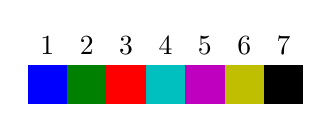
\begin{tikzpicture}[scale=0.5]
        \foreach \x/\c in {1/bb, 2/gg, 3/rr, 4/cc, 5/mm, 6/yy, 7/kk} {
            \fill[\c] (\x, 0) rectangle ++(1,1);
            \path (\x,1) ++ (right:0.5) node[above] {\x};
        };
    \end{tikzpicture}
    \caption{Color order for sweep plots in the report.}
    \label{fig:colororder}
\end{figure}

When two-port S-parameter measurements are mentioned in the report, port 1 is always the top-antenna and port 2 is the side-antenna unless otherwise noted.

